\documentclass{llncs}
\RequirePackage[T1]{fontenc}
\usepackage[cp1250]{inputenc}

\usepackage{pgf}
\usepackage{tikz}
\usepackage{listings}
\usepackage{url}
\usepackage{xspace}
%\numberofauthors{3}
\author{
%\alignauthor
J�drzej Fulara and
%\affaddr{Institute of Informatics}\\
%\affaddr{University of Warsaw}\\
%\affaddr{ul. Banacha 2}\\
%\affaddr{02-097 Warsaw, Poland}\\
%\email{fulara@mimuw.edu.pl}
%\alignauthor
Krzysztof Jakubczyk and
%\affaddr{Institute of Informatics}\\
%\affaddr{University of Warsaw}\\
%\affaddr{ul. Banacha 2}\\
%\affaddr{02-097 Warsaw, Poland}\\
%\email{kjk@mimuw.edu.pl}
%\alignauthor
Aleksy Schubert
%\affaddr{Institute of Informatics}\\
%\affaddr{University of Warsaw}\\
%\affaddr{ul. Banacha 2}\\
%\affaddr{02-097 Warsaw, Poland}\\
%\email{alx@mimuw.edu.pl}
}
\bibliographystyle{abbrv}
\title{Supplementing Java Bytecode with Specifications}

\newcommand{\jmltobmltext}{JML2BML}
\newcommand{\jmltobml}{\textsl{\jmltobmltext}\xspace}
\newcommand{\openjml}{OpenJML\xspace}
\newcommand{\bmllib}{BMLLib\xspace}
\newcommand{\hs}{\hspace{0.5pt}}


\lstdefinelanguage{BML}{morekeywords={abstract,break,byte,case,catch,char,class,%
      const,continue,default,do,double,else,extends,false,final,%
      finally,float,for,goto,if,implements,import,instanceof,%
      interface,label,long,native,new,
      boolean, int,%
      null,%
      package,private,protected,public,ghost,%
      return,short,static,super,switch,synchronized,this,throw,%
      throws,transient,true,try,void,volatile,while,
      requires,precondition,ensures,exsures,exists,forall,&&,%
      old_this,loop_inv,\result,\everything,\nothing,%
      loop_specification,modifies,invariant,decreases,%
      iconst_0,iconst_1,istore_3,iinc,iload_3,%
      aaload,aload_0,aload_1,aload_2,aastore,%
      if_acmpne,if_icmplt,%
      invokespecial,getfield,%
      arraylength,ireturn},%
   sensitive,%
   morecomment=[l]//,%
   morestring=[b]",%
   morestring=[b]',%
    basicstyle=\small,
    keywordstyle=\bfseries\color{black},
    commentstyle=\itshape\color{blue},
    mathescape=true,
}


\begin{document}
\maketitle


%\section{What should be in paper}
%\begin{itemize}
%	\item What is JML
%	\item What is BML
%	\item Why is translation needed??
% \item Why the tool needed?? (JVM -> VM) BML can be used to different languages, JML to one??
%	\item The tool isn't built on any existing comipler.
%	\item As input we get source file with JML annotations and compiled class file.
%	\item Therefore we can't used optimised bytecode (problem with loops, assertions etc.)
%	\item Optimized bytecode may be used for more general annotations eg. method invariants.
%	\item Detecting loops in bytecode
%	\item Description of matching source code with bytecode loops
%	\item Non-trivial example
%\end{itemize}
%\maketitle

\begin{abstract}
Java class file is an interoperable format that can serve not only to
transfer the compiled versions of Java programs, but also to embed
into the files additional information which can be exploited by the
execution environment of user's machine to speed up the execution of
the application or to ensure certain vital properties of the code. The
latter goal is specifically the aim of the proof-carrying code (PCC)
techniques in which the executable code is supplied with a proof that
the code obeys certain policy (e.g. the program does not store
password in clear in a file). BML (Bytecode Modelling Language) can
be regarded as a part of the PCC architecture which allows to express
detailed properties of bytecode programs, in particular the policies
they must obey.

As most of the programming is done at the source code level, it is
desirable to have a way to translate properties expressed at the
source code level (in our case written in Java Modeling Language, JML)
to the bytecode level.  In this paper we present a \jmltobml
compiler, a tool that for a given Java source file annotated with
specifications generates class files with BML.
\end{abstract}
%# Alternative languages on the Java VM
%# Java Extensions
%#  - PCC
%#  Optimization
%#  - PCC
%# VM Design
%# Java Verification
%#  - PCC
%#Java for Embedded Systems
%*   Middleware for Mobile Applications
%* Location-Based Services
%* M-Business Applications
% page limit: 10 pages

%\category{D.2.4}{Software Engineering}{Software/Program Verification}

%\terms{Reliability, Verification}

%\keywords{Java, bytecode, JML, BML} % NOT required for Proceedings

\section{Introduction}

Each Java Virtual Machine is required to perform so called bytecode
verification process on each class file which is loaded to be executed
\cite{verification}. This verification process ensures vital
properties of the loaded programs such as that all arguments on the
operand stack are legal, all types of variables passed to methods are
correct, all load and store operations have correct types, etc.

In certain situations, these guarantees are not sufficient. In
particular, many of the current security guarantees are ensured at
runtime of an application. For instance, a mobile application asks the
user to acknowledge the sending of data over the mobile
network. However, the user may get bored with many such prompts and
disable this security property. After this, she or he may easily be
made to send data to e.g. an expensive premium number. In this case,
it would be more secure to give the user a load- (or download-) time
guarantee that the code sends data only to expected receivers.
Currently, this is partially done through digital signatures. The
signatures, however, do not assure that the software is indeed
secure. They only certify who takes (not so well defined)
responsibility for the problems caused by the program.  In fact, there
were cases when many users were deceived by respected companies
e.g. rootkits were installed when audio CD was inserted \cite{BMGcase}.

Another guarantee which is not secured by the traditional bytecode
verification procedure is the lack of code inconsistencies typically
considered to be programming errors i.e. null-pointer exceptions,
array index out of bounds exceptions etc. In many cases, these
inconsistencies can be eliminated with the help of some additional
information (e.g. @NonNull annotations, suggested in \cite{JSR305})
which makes the checking process feasible.

The goal of the proof-carrying code (PCC) technique
\cite{pcc,PCCForJava} is to give the user certain guarantees of the
code to be executed at the moment of its execution. In this paradigm,
the executable code (in case of Java, the bytecode) is augmented with
an additional piece of information, a PCC certificate, which together
with the code makes possible an automatic check that the code indeed
obeys the expected policy (e.g. sends data to authorised targets
only). This check is performed by the user (or by user's execution
environment) right before the code is executed (see
Figure~\ref{fig:pccScheme}). In fact, the usual Java bytecode
verification procedure can be viewed as an example of a forerunner of
this technique \cite{LightweightBytecodeVerification}. Although the
certificate is in this case empty (or supplementary in case the
StackMap attributes are employed), the execution environment indeed
checks a vital code property before the code is executed. In more
complicated cases of the proof-carrying code, one needs additional
information to make the checking of the required property feasible or
even algorithmically possible.

One of the possible ways to realise the PCC architecture is developed
under the European project MOBIUS.\footnote{See
\url{http://mobius.inria.fr}} This project plans to develop both
type-based and logic-based PCC program certification techniques
\cite{MOBIUSscenarios}. The logic-based methods rely on specification
of the object-oriented code in the fashion governed by the
design-by-contract principles \cite{DesignByContract}. Bytecode
Modeling Language (BML) is a specification language which realises the
methodology at the bytecode level \cite{bmlBurdy}. It is designed as a
counterpart of the Java Modeling Language (JML), an established
specification language dedicated to formally describe properties of
Java programs in the design-by-contract style \cite{JML}.

\begin{figure}
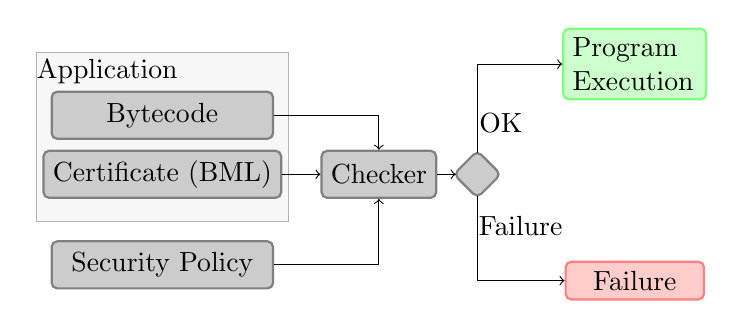
\begin{tikzpicture}[scale=0.5]

\tikzstyle{vertex}=[rectangle,draw=black!50,fill=black!20,thick,rounded corners = 2pt, minimum width=80pt, minimum height=17pt]
\tikzstyle{vertex2}=[rectangle,draw=black!50,fill=black!20,thick,rounded corners = 2pt, minimum height=17pt]
\tikzstyle{vertex3}=[rectangle,draw=green!50,fill=green!20,thick,rounded corners = 2pt, minimum width=50pt, text width=45pt]
\tikzstyle{vertex4}=[rectangle,draw=red!50,fill=red!20,thick,rounded corners = 2pt, minimum width=50pt]

\tikzstyle{rotated}=[rectangle,draw=black!50,fill=black!20,thick,rounded corners = 2pt,rotate=45, minimum height=12pt, minimum width = 12pt]
\tikzstyle{rl}=[line join = round]
\filldraw[draw=black!30,fill=black!3] (-3.2,3.8) rectangle (3.2,-0.5);
\node (app) at(-1.4,3.3) {Application};
\node[vertex] (bytecode) at (0,2.2){Bytecode};
\node[vertex] (certificate) at (0,0.7) {Certificate (BML)};

\node[vertex](policy) at (0, -1.6) {Security Policy};

\node[vertex2](checker) at (5.5,0.7) {Checker};
\node[rotated](rot) at (8, 0.7) {};
\node[vertex3](execution) at (12,3.5) {Program Execution};
\node[vertex4](failure) at (12,-2) {Failure};
\draw[->] (certificate) to[out=0,in=180] (checker);
\draw[->] (checker.east) -- (7.45,0.7);
\draw[->] (bytecode.east) -- (5.5,2.2) -- (checker.north);
\draw[->] (policy.east) -- (5.5,-1.6) -- (checker.south);
\draw[->] (8,1.25) -- (8,3.5) -- (execution.west);
\draw[->] (8,0.15) -- (8,-2) -- (failure.west);
\node (ok) at (8.6, 2) {OK};
\node (ok) at (9.1, -0.6) {Failure};
\end{tikzpicture}
\caption{Proof-Carrying Code architecture for bytecode.}
\label{fig:pccScheme}
\end{figure}

The use of specification formalisms such as JML or BML has another
important application. Modern, high level programming languages
support creating software in a modular way. Applications can be
divided into smaller parts that can be developed independently. In
large systems, it is a common practice to outsource some well defined
subsystems to external companies. The main problem in this approach is
that the pieces of software developed by different programming teams
often are not fully compatible. To avoid this incompatibility and
useless code that is produced, there is a need to specify precisely
the desired behaviour of the components, what they require and what
can we expect from them \cite{SoftwareReuse}. The solution is to
define formally implementation contracts in languages such as JML or
BML and check automatically the compliance of the code with these
descriptions.

Specification languages are useful in describing the system components
behaviour. They are not only helpful in dividing the problem into
smaller pieces, but also focus on \textit{what} is expected from each
part, without saying about \textit{how} should it be done. The
specification languages are designed to be simple enough to be
understood by programmers, so they can play the role of code
documentation. Using specification language for documenting code has
the advantage that it is possible to automatically verify that the
source code implements the documented features
\cite{formalDocumentation}.

The distributed development of software results in a situation where
different software modules are implemented in different
languages. This is facilitated by the fact that more and more
languages are compiled to the same Java bytecode. A few examples:
\begin{itemize}
\item Jython: the Python Java implementation,
\item JRuby: the Ruby Java implementation,
\item Jacl: the Tcl Java implementation,
\item Rhino: the JavaScript Java implementation,
\item Scala: a functional programming language compiled to
  Java bytecode.
\end{itemize}
At SugarCon 2008, Sun Microsystems President and CEO Jonathan Schwartz
said "we are just going to take the 'J' off the 'JVM' and just make it
a 'VM'". Therefore there will be a global trend with support of
companies to use JVM with languages other than Java.  This is an
important reason, why it is significant to be able to translate the
source code specifications into lower level language
specifications\hs{}---\hs{}in case the development is done in many
languages the only common platform is the platform of the executable
code. This explains the efforts concerning BML specification language.

The JML specification language exists already for several years. In
the course of the time, a lot of code have been annotated with the
specifications in this language (see \cite{overviewOfJML} for an
overview). Except for that, it is easier to understand and specify the
code in the source form than in the bytecode form. In this light, it
is desirable to translate these specifications from JML to
BML. Moreover, the code producer in PCC scenarios, who has to produce
a correctness proof, will often prefer to construct it rather in terms
of the source code than in terms of the bytecode, and then compile the
specification and the proof into the level of executable code.

In a broader perspective, the full infrastructure to support the use
of BML annotated programs, for which complicated properties are
checked at the user's end, requires the following items:
\begin{itemize}
\item PCC checker tools that understand BML annotations combined with
  PCC certificates,
\item tools which enable the construction of PCC certificates,
\item procedures to safely distribute the desired properties to be
  checked by PCC infrastructure,
\item modelling languages (such as JML for Java) for other programming
  languages,
\item compilers that compile programs to JVM bytecode along with
  annotation compilers.
\end{itemize}
The \jmltobml compiler described in this paper is designed to be a
part of this scheme which translates the policies and specifications
to the bytecode format.


\paragraph{Organisation of the paper}
In Section~\ref{sec:specification}, we present the specification
languages JML and BML. An example which illustrates the work of the
compiler is presented in Section~\ref{sec:example}.
Section~\ref{sec:compiler} overviews the design of the \jmltobml
compiler. The most difficult problem of the specification compilation
is the placement of the loop invariants. This issue is discussed in
Section~\ref{sec:loops}. The related work is presented in
Section~\ref{sec:related-work} and we conclude in
Section~\ref{sec:conclusion}.


\section{Specification Languages}
\label{sec:specification}

\subsection{JML}
The Java Modelling Language (JML) is a behavioural specification
language for Java programs \cite{JML}. It allows to write
specifications according to the \textit{design-by-contract} principles
\cite{DesignByContract}. Data types and method behaviour can be
precisely commented using JML annotations. They describe the invariant
properties that are maintained by objects, the input method
requirements (preconditions), what we can expect at the output of
method (postconditions) and also some lower level properties of the
code (i.e. loop invariants, loop variants etc). JML annotations are
written in standard Java comments, so they do not affect the normal
work of any Java compiler.

An important goal in the design of JML is that it should be easily
understandable by Java programmers. It is achieved by staying as close
as possible to the Java syntax and semantics. The tool support for JML
is rich (see \cite{overviewOfJML} for an overview). In particular,
there are tools that check JML specification at runtime
\cite{runtime}, in extended static checking fashion \cite{escJava},
and allow to perform software certification \cite{krakatoa}. There are
also tools that support annotation generation
\cite{canapa,daikon}.

The works on JML was started by Gary Leavens at Iowa State
University. Since then it became an open project, multiple groups
around the world are writing tools supporting JML and developing the
language itself.

\subsection{BML}
The Bytecode Modelling Language (BML) is a specification language for
the bytecode. It was proposed by Burdy et al. in \cite{bmlBurdy}. The
design of BML directly follows the fundamental concepts of JML. It
inherits most constructions and keywords from the JML syntax. As the
BML is developed within the MOBIUS \cite{mobius} project and the main
target of the project are Java-enabled mobile devices such as mobile
phones, the current version of BML assumes some simplifications of the
Java bytecode which are present in the J2ME platform\hs{}---\hs{}the Java
platform for mobile devices with restricted resources.

The class files representing bytecode with BML annotations are regular
Java class files, executable by all Java tools. The annotations are
stored within additional attributes. The BML related attributes start
with the prefix \texttt{org.bmlspecs} and according to the
specification of the Java Virtual Machine they should be ignored by
the Machine, since their names are not part of the original JVM
specification.

Of course, following the logical structure of class files, class
specifications are stored as class attributes, method specifications,
as attributes of corresponding method and specifications inserted in
the code are attributes of the JVM Code attribute of the given method.

%The document is organized as follows. In Section 2 we describe an
%annotation language. In Section 3 we describe implementation of our
%compiler, give details on the architecture and present the main
%principles of the translation. Then an example of using our tool is
%presented. In Section 5 and 6 we describe algorithms for detecting
%loops in the bytecode and matching them with the source code. At the
%end conclusions are given and future work is discussed.

\subsection{Overview of Annotations}

The structure of annotations in BML and JML is very similar. We have
two main types of annotations: method annotations and data type (class
and interfaces) annotations.

\subsubsection{Method annotations}
The most important type of method annotations are \textit{method
specifications} describing the input-output behaviour of the
method. This are preconditions (\texttt{requires}), defining
conditions that should be fulfilled before entering the method and
postconditions (\texttt{ensures}) telling what we can expect after the
method finishes. One can define also which fields are modified (clause
\texttt{modifies}) and which exceptions might be thrown (clause
\texttt{signals}).

The other type of method annotations are specifications elements
appearing in the code, like:
\begin{itemize}
\item {Assert instructions that state some facts about fields,
  variables etc. that should hold at this point of program execution.}
\item {Loop specifications that describe the loop invariants
  (\texttt{loop\_invariant}), loop variants, like \texttt{decreases} to
  prove the loop's termination or \texttt{modifies} that tells which
  fields or variables can be changed in this loop.}
\item{Declarations of local \texttt{ghost}
  variables\hs{}---\hs{}variables that exist only in the
  specification. Their values can be modified only using special
  \texttt{set} instructions.}
\item{\texttt{Set} instructions are similar to Java assignments, but
  they operate on ghost fields and variables.}
\end{itemize}

\subsubsection{Data type annotations}
Class (and interface) specifications describe the behaviour of a class
as a whole (in the \texttt{static} version) or of objects of that
class (\texttt{instance}). The most important type of \textit{class
specifications} are class invariants. They describe the property that
should hold for all objects of this class in all \textit{visible}
states, i.e. after all constructors and before and after all
methods. For example, having a field \texttt{Object[] list}, one can
write an invariant that the list is never null and its length is
10. Class invariants can be seen as additional, implicit preconditions
and postconditions for all methods in the class.

Other important class specifications are:
\begin{itemize}
\item {Declarations of \texttt{ghost} fields. They are similar to
  local ghost variables, but are visible in the whole class scope.}
\item {Model fields\hs{}---\hs{}fields present only in the specifications,
  representing some more complicated formulae. For example one can
  create a model field representing the property that a collection does
  not contain nulls.}
\end{itemize}
More details can be found in \cite{jmlrefman} and \cite{bmlrefman}.

\lstset{language=java, morekeywords={requires,ensures,\result,\exists,\old,loop_invariant,\forall,==>, decreases},
        basicstyle=\scriptsize,commentstyle=\scriptsize,moredelim=*[s][\scriptsize]{/*@}{*/},
        numbers=left,numberstyle=\tiny,stepnumber=4,numbersep=5pt}
\begin{figure}[htbp]
~~~~~~%
\begin{minipage}{400pt}
\begin{lstlisting}
public class List {

  private Object[] list;

  /*@ requires list != null;
    @ ensures \result ==(\exists int i;
    @ 0 <= i && i < list.length &&
    @ \old(list[i]) == o1 && list[i] == o2);
    @*/
  public boolean replace(Object o1, Object o2){
    /*@
      @ loop_invariant i <= list.length
      @ && i >=0 && (\forall int k;0 <= k
      @ && k < i ==> list[k] != o1);
      @ decreases list.length - i;
      @*/
    for (int i = 0; i < list.length; i++) {
      if (list[i] == o1) {
        list[i] = o2;
        return true;
      }
    }
    return false;
  }
}
\end{lstlisting}
\end{minipage}
\caption{An example class \texttt{List.java} containing single method
\texttt{replace}.}
\label{fig:source}
\end{figure}

\section{An Example of Using The\\Compiler}
\label{sec:example}

This section provides an example demonstrating the result of launching
the \jmltobml.
\subsection{Source Code}
Consider the class presented on Figure~\ref{fig:source}. This is an
excerpt of a class which implements a sequence of objects. We present
here only one method that replaces in the \texttt{list} array the
first occurrence of its first parameter with the second one. True will
be returned, if and only if such an element was found.

The presented code, apart from standard Java statements, contains also
specifications in the JML. There is a precondition (\texttt{requires
...}) for the method \texttt{replace} defined. It requests that every
time the method is invoked, the field \texttt{list} it not
\texttt{null}\footnote{In general a method can have multiple
\texttt{requires-ensures} pairs. In this case the method can be
invoked only in places where at least one of the conditions specified
\texttt{requires} clauses holds.}. The next three lines (starting with
\texttt{ensures}) constitute the method postcondition. It states that,
if the precondition was fulfilled, then the method result is true if
and only if there was an element in the \texttt{list} which value has
been updated from \texttt{o1} to \texttt{o2}. Note that the
postcondition makes use of some JML features, like
\texttt{$\backslash$result}, \texttt{$\backslash$old} or
\texttt{$\backslash$exists}. This postcondition does not describe all
properties of this method. For example an implementation that replaces
all elements in the \texttt{list} up to the first occurrence of
\texttt{o1} with \texttt{o2} will fulfil this specification.

In addition to specification describing input-output beha\-viour of
the method, also the loop implementing the \texttt{replace} method is
annotated. The \texttt{loop\_invariant} clause contains the invariant:
a formula that should hold at the beginning of the loop body at each
loop iteration. In this example it states that in iteration \texttt{i}
there are no occurrences of \texttt{o1} in \texttt{list} on positions
before \texttt{i}. The annotation \texttt{decreases} describes the
loop variant. It specifies an expression (in this case
\verb|list.length - i|) which value is decreased in each loop
iteration by at least one.

\subsection{Bytecode}
In this section we describe the result of translating the source code
from Figure~\ref{fig:source}. The actual result of the compilation is
a class file enriched with the attributes which contain the
representation of BML specifications. This means that the binary class
files are not human readable. Thus, we rely for the current
presentation on its textual representation obtained from the
\bmllib. The Figure~\ref{fig:bytecode} shows the translated
\texttt{replace} method together with BML annotations inserted by our
\jmltobml compiler. The bytecode instructions labelled with 0 and 1
correspond to the initialisation \texttt{i = 0}. The loop is located
between lines 2 and 33. Lines 5--12 represent the \texttt{if}
statement, 15--23 correspond to lines 19--20 from the source
code. Loading loop condition parameters is located in lines 27--32 and
33 performs the loop condition comparison.

The \texttt{requires-ensures} pair is translated into input-output
behaviour BML specifications located just before the method code. We
can see that the BML code contains two places where the counterpart of
the JML \texttt{requires} clause can be placed. The first one is right
after the \texttt{requires} keyword and the second one is after the
\texttt{precondition} keyword. In fact, both JML and BML allow one to
specify many pairs of the input-output specifications. The semantics
of the multiple pairs is such that for each pair where the requires
formula holds at the entry to the method, the corresponding ensures
formula must hold at the exit (so effectively the conjunction of all
these ensures formulae must hold). However, we often want to specify
that a particular method can be called only in specific context
(e.g. with first parameter being non-null) and except for that it
should obey the input-output behaviour described in multiple
\texttt{requires-onuses} pairs. In this situation, it is more
convenient to distinguish a single additional clause which should hold
in all the cases instead of copying to all the pairs. In our JML code,
this clause is implicit and equivalent to \texttt{true} whereas in BML
this is made explicit as the formula after the \texttt{requires}
keyword. This is also why the actual JML precondition is translated to
the internal \texttt{precondition} statement (it is one, and in this
particular instance the only one, of potentially many preconditions).

Loops specifications are located after the line labelled with~32 in
the presented listing. The \jmltobml compiler detects loops in the
bytecode and inserts the annotation before the statement representing
the beginning of a loop condition. In this case it is the
\texttt{if\_icmplt} instruction comparing \texttt{i} and
\texttt{list.length}. (For more details about detecting loops see
Section~\ref{sec:loops}.) The modifies clause describes set of
variables modified by the loop. We can see it in the listing as this
clause is obligatory in BML. Currently, because of \openjml
limitations, it is not supported by our compiler (the default value
\texttt{everything} will be inserted) so we see the default value
inserted at this point.

%\newpage

\begin{figure}[htbp]
\lstset{language=bml}
\lstset{basicstyle=\small,stepnumber=400,numbersep=5pt}

~~~~~~%
\begin{minipage}{400pt}
\begin{lstlisting}
/*@
  @ requires true
  @  {|
  @   precondition list != null
  @   ensures \result ==
  @     (\exists int i; 0 <= i &&
  @              i < list.length &&
  @              old_list[i] == o1 &&
  @              list[i] == o2)
  @  |}
  @*/
public boolean replace(Object o1, Object o2)
0:    iconst_0
1:    istore_3
2:    goto	   #27
5:    aload_0
6:    getfield	   main.List.list
9:    iload_3
10:   aaload
11:   aload_1
12:   if_acmpne	   #24
15:   aload_0
16:   getfield	   main.List.list
19:   iload_3
20:   aload_2
21:   aastore
22:   iconst_1
23:   ireturn
24:   iinc	   %3	1
27:   iload_3
28:   aload_0
29:   getfield	   main.List.list
32:   arraylength
/*@
  @ loop_specification
  @   modifies everything
  @   invariant i <= list.length &&
  @      i >= 0 &&
  @      (\forall int k; 0 <= k &&
  @          k < i ==> list[k] != o1)
  @   decreases list.length - i
  @*/
33:   if_icmplt	   #5
36:   iconst_0
37:   ireturn

\end{lstlisting}
\end{minipage}
\caption{The method \texttt{replace} in the \texttt{List.class}}
\label{fig:bytecode}
\end{figure}

\section{\jmltobmltext{} Compiler Design}
\label{sec:compiler}

\jmltobml takes as input a Java source file with JML annotations
together with the corresponding class file and outputs the class file
with inserted proper BML annotations. Our compiler uses an enhanced
Abstract Syntax Tree (AST) for the Java source code, taken from the
\openjml\footnote{Available from
\url{http://sourceforge.net/projects/jmlspecs}} compiler (a Java
compiler with JML checker based upon the OpenJDK Java tool set). For
different types of JML clauses, there are separate translation rules
defined. At each node of the AST, all translation rules are
applied. If some rule succeeds to translate this node, the result is
stored in the class file, using the \bmllib library
\cite{bmllib}. This approach makes the compiler easily extensible. It
is enough to just write a new translation rule to support additional
features of the JML language. Moreover, the acyclic structure of the
code should make the future maintenance more feasible and facilitate
the understanding of the code mechanisms by future contributors
\cite{Dijkstra70}.

Currently, the \jmltobml compiler focuses on a subset of the JML
called JML Level 0. Due to external libraries limitations not all
desired features are translated, for example the
loop \texttt{modifies} clause is not supported by \openjml. The
\jmltobml compiler is designed to be compatible with other bytecode
level tools, such as the bytecode editor \textit{Umbra}.

\subsection{Architecture Description}

In this section we present the overview of the architecture of
\jmltobml compiler. The \jmltobml compiler uses \openjml to parse the
Java source code together with the JML annotations. To insert
generated BML annotations, the \bmllib library is used. The
dependencies between internal packages of \jmltobml and \openjml and
\bmllib are presented on Figure~\ref{fig:packages}.

The \texttt{jml2bml.main} package provides the entry point to the
application. JML annotations from given source file will be translated
and inserted into corresponding class file. Functions to access some
bytecode information are located in \texttt{jml2bml.bytecode} and
helpers to \bmllib are collected in \texttt{jml2bml.bmllib}. The
\texttt{jml2bml.rules} package contains translation rules for
different aspects of JML. It should be easy to add new rules in the
future. Classes for traversing the Java abstract syntax tree can be
found in \texttt{jml2bml.ast}. In \texttt{jml2bml.symbols}
implementation of the symbol table, which is used in the translation
of JML to BML, can be found. The \texttt{jml2bml.engine} package
contains the core translation mechanism.
\begin{figure}[ht]
\centering{
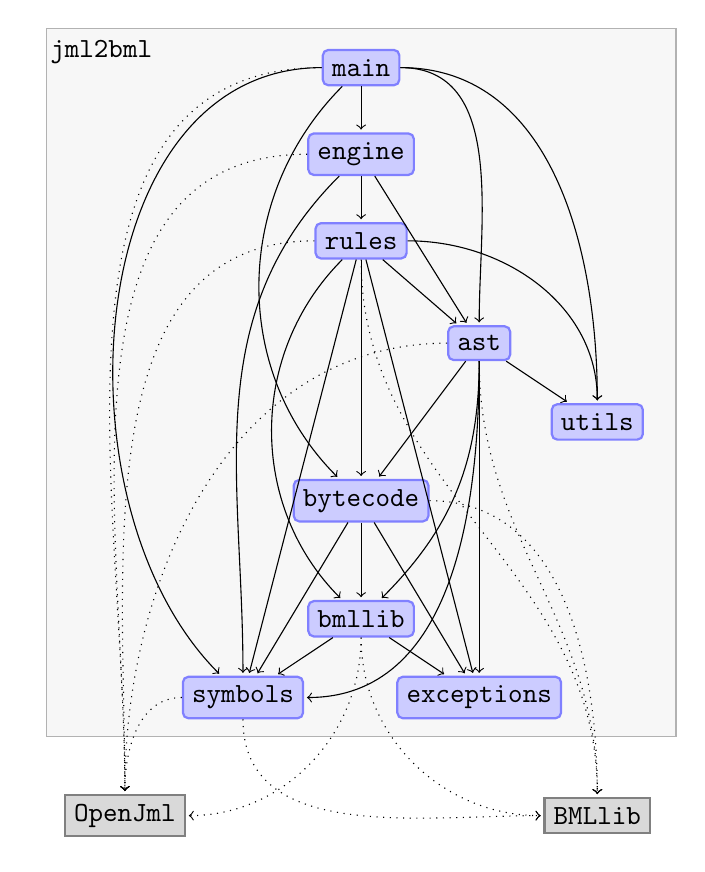
\begin{tikzpicture}[shorten >=1pt,->]
\
\tikzstyle{vertex}=[rectangle,draw=blue!50,fill=blue!20,thick,rounded corners = 2pt]
\filldraw[draw=black!30,fill=black!3] (-1,7.5) rectangle (7,-1.5);
%\draw (-0.9,7.2) node[right]{\textbf{\texttt{jml2bml}}};
\node (label) at (-0.3,7.2){\texttt{jml2bml}};
\node[vertex] (main) at (3,7) {\texttt{main}};
\node[vertex] (engine) at (3,5.9) {\texttt{engine}}  ;
\node[vertex] (rules) at (3,4.8) {\texttt{rules}}  ;
\node[vertex] (ast) at (4.5,3.5) {\texttt{ast}}  ;
\node[vertex] (utils) at (6,2.5) {\texttt{utils}};
\node[vertex] (bytecode) at (3,1.5) {\texttt{bytecode}};
\node[vertex] (bmllib) at (3, 0) {\texttt{bmllib}};
\node[vertex] (exceptions) at (4.5, -1) {\texttt{exceptions}};
\node[vertex] (symbols) at (1.5, -1) {\texttt{symbols}};
\draw (main) -- (engine);
\draw (engine) -- (rules);
\draw (rules) --(ast);
\draw (engine) -- (ast) ;
\draw(ast) -- (utils) ;
\draw(ast) -- (bytecode);
\draw (ast) to[out=270,in=45] (bmllib);
\draw (ast) -- (exceptions);
\draw (main) to[out=0,in=90] (ast);
\draw (rules) to[out=0,in=90] (utils);
\draw (rules) -- (symbols);
\draw (rules) -- (exceptions);
\draw (rules) to[out=225,in=135] (bmllib);
\draw (main) to[out=0,in=90] (utils);
\draw (main) to[out=225,in=135] (bytecode);
\draw (main) to[out=180,in=135] (symbols);
\draw (engine) to[out=225,in=90] (symbols);
\draw (ast) to[out=270,in=0] (symbols) ;
\draw (rules) -- (bytecode);
\draw (bytecode) -- (bmllib) ;
\draw (bytecode) -- (exceptions) ;
\draw (bytecode) -- (symbols) ;
\draw (bmllib) -- (exceptions) ;
\draw (bmllib) -- (symbols) ;
\tikzstyle{external}=[rectangle,draw=black!50,fill=black!15,thick]
\node[external] (BmlLib1) at  (6, -2.5) {\texttt{BMLlib}};
\node[external] (openJml) at  (0, -2.5) {\texttt{OpenJml}};
\draw[dotted] (main) to[out=180,in=90] (openJml);
\draw[dotted] (engine) to[out=180,in=90] (openJml);
\draw[dotted] (rules) to[out=180,in=90] (openJml);
\draw[dotted] (rules) to[out=270,in=90] (BmlLib1);
\draw[dotted] (ast) to[out=270,in=90] (BmlLib1);
\draw[dotted] (ast) to[out=180,in=90] (openJml);
\draw[dotted] (bytecode) to[out=0,in=90] (BmlLib1);
\draw[dotted] (bmllib) to[out=270,in=0] (openJml);
\draw[dotted] (bmllib)  to[out=270,in=180] (BmlLib1);
\draw[dotted] (symbols) to[out=180,in=90] (openJml);
\draw[dotted] (symbols) to[out=270,in=180] (BmlLib1);
\end{tikzpicture}
}
\caption{The dependency graph of the \jmltobml packages. Dotted lines denote access to external libraries.}
\label{fig:packages}
\end{figure}
\subsection{Translation Mechanism}
The full translation consists of a set of independent translation
rules. Having the set of rules the AST tree of the source code with
annotations is traversed. For each visited node all translation rules
are applied. For most nodes translation rules do
nothing\hs{}---\hs{}each is responsible for a few node types. The
translation mechanism allows to register new rules in a very simple
way. This is an important issue in case as we predict that new
features will be added both to JML and BML.

\subsubsection{Translation rules}
The \jmltobml compiler uses a set of translation rules. The concept of
translation rule is that it should be responsible for relatively
small, independent piece of translation. For example we have separate
rule for translating \textit{assert} and another one for translating
\textit{loop\_invariant}. Each rule is responsible for translation of
a part of the AST tree resulting from a particular non-terminal of the
input grammar. Translation rule may write results of translation to
the output class file (using \bmllib). It can, however, only collect
some translated data that may be used by other translation rules. For
example both\hs{}---\hs{}the \textit{assert} and
\textit{loop\_invariant} annotations contain expressions. Therefore we
created an expression translation rule that makes translation of an
expression but it does not write anything to output
file\hs{}---\hs{}just returns the translated expression that will be
used in other translation rules.

It is relatively easy to extend translation using the translation rule
concept. For example if we would like to translate an annotation that
was not already translated we should create a new translation rule
implementation and include it in the translation mechanism by
registering the rule in the translation manager. When implementing the
translation rule we should first find out which AST nodes are relevant
to the implemented translation operation and then override proper
methods of the base skeletal class, \texttt{TranslationRule<String>}.
The default methods from the skeletal class do nothing, so the methods
which are not overridden will just represent identical translation for
the case they represent.

Translation rule key design features are:
\begin{itemize}
\item the concept falls into a visitor design pattern,
\item translation rule is an extension of a simple abstract class,
\item translation process can be broken into smaller, independent pieces,
\item extending translation is simple.
\end{itemize}

\subsubsection{Example of a translation rule}

\newcommand{\Tr}{\mathrm{Tr}\xspace}
\newcommand{\invariantkeyword}{\mathsf{invariant\_keyword}\xspace}
\newcommand{\predicate}{\mathsf{predicate}\xspace}
\newcommand{\translationcontext}{\mathsf{translation\_ctxt}\xspace}
\newcommand{\JAST}{\mathsf{JMLAST}\xspace}
\newcommand{\TContext}{\mathsf{Ctxt}\xspace}
\newcommand{\replace}{\mathrm{replace}\xspace}
\newcommand{\getInvariant}{\mathrm{getInvariant}\xspace}
\newcommand{\getInvExpression}{\mathrm{getInvExpression}\xspace}
\newcommand{\getExpression}{\mathrm{getExpression}\xspace}
\newcommand{\packInvariant}{\mathrm{consInvariant}\xspace}
We present here a rule which translates a JML invariant into a BML
invariant. The main non-trivial work of the rule is to combine all the
JML invariants in the current class into a single invariant in the
resulting BML representation (the specification in BML can contain
only one instance invariant for a single class).

The logic of the translation rule can be described in an abstract way
as follows:
\begin{displaymath}
\begin{array}{l}
\Tr(\invariantkeyword\; \predicate, \translationcontext) =\\
\quad    \replace(\translationcontext, \\
\quad\quad   \getInvariant(\translationcontext),\\
\quad\quad   \packInvariant(\\
\quad\quad\quad   \getInvExpression(\\
\quad\quad\quad\quad \getInvariant(\translationcontext))\;\&\&^*\\
\quad\quad\quad   \getExpression(\Tr(\predicate, \translationcontext ))))
\end{array}
\end{displaymath}
where $\Tr : \JAST \times \TContext\to \TContext$ is the function
which defines the translation. It takes a JML AST node and a
translation context and transforms this into a new translation context
which contains the result of the translation.

The $\replace$ function replaces in the given translation context the
item from the second argument with the item on the third argument. In
our case, it replaces the current invariant (obtained using the
$\getInvariant$ function from the current context) with the newly
generated one. The newly generated invariant is constructed (using
$\packInvariant$) from the conjunction of the expression obtained from
the already accumulated invariant (obtained using $\getInvExpression$)
with the expression being the result of the translation of the
predicate in the currently translated invariant ($\predicate$). One
remark must be made about the operation of the conjunction. In case
the first argument is undefined (it happens when we translate the
first invariant in the class), the operation $\&\&^*$ results just in
its second argument.

Figure~\ref{fig:translation_rule_example} contains the Java code which
implements the above described translation rule. The rule directly
extends the base \texttt{TranslationRule} class.  It has one attribute
\texttt{context}, which holds the context in which rule will be
executed. Class invariants in OpenJML abstract syntax tree are
represented by \texttt{JmlTypeClauseExpr} class nodes. As we use
visitor pattern, we have to override method responsible for these
nodes, \texttt{visitJmlTypeClauseExpr}.

Implementation of the translation method is simple. First we check if
this is the node type we are interested in, line \ref{rule_token}. We
get an object representing the class which we want to add invariant to
(line \ref{rule_class}). Next, in line \ref{rule_formula}, we
translate the content of invariant\hs{}---\hs{}the rule which
translates the expression is used here. In line
\ref{rule_get_invariant}, the existing class invariant is retrieved
from the class. If there is no invariant, a new one is created (line
\ref{rule_new_invariant}), otherwise we combine an old invariant
formula with the new one using the \texttt{\&\&} logical connective
(line \ref{rule_new_formula}). The result is fed to a new class
invariant in line \ref{rule_update_invariant}. At the end, in line
\ref{rule_set_invariant} we set new invariant to the class.


%The translation rule is a very simple but powerful concept. It uses a visitor design pattern.
%Before running the translation mechanism, translation rules need to be registered. Abstract syntax tree of the source code is traversed and for each node translation rules are executed.
%The whole tree is traversed and in each node all defined translation rules are applied. It allows also to register new rules in a very simply way, what is an important issue in case of implementing new features in the future.

\subsection{Translating Expressions}
In order to be able to translate any JML specification, one needs to
translate JML expressions, so one of the most substantial tasks in
writing the compiler was to write a translation rule for
expressions. The syntax of JML expressions follows the one of Java
expressions which makes them easily accessible for typical Java
programmers. That is also why the BML expressions are similar to JML
ones and include:
\begin{itemize}
\item{Binary arithmetic operations (\verb!+!, \verb!-!, \verb!*!,
  \verb!/!)}
%\end{itemize}
%\begin{itemize}
\item{Boolean operations}
\item{Relational operators ($<$, $\le$, $\ge$, $!=$, etc.)}
\item{Logical formulae containing
  \begin{itemize}
  \item special expressions such as reference to old value (\verb!\old!),
    reference to the result of method (\verb!\result!),
  \item implications, conjunctions, alternatives, etc.,
  \item quantifiers (with bound variables).
\end{itemize}}
\end{itemize}
\lstset{language=java,
        basicstyle=\scriptsize,commentstyle=\scriptsize,moredelim=*[s][\scriptsize]{/*@}{*/},
        numbers=left,numberstyle=\tiny,stepnumber=4,numbersep=5pt,escapeinside={(*@}{@*)}}
\begin{figure}[htb]
~~~~~~%
\begin{minipage}{220pt}
\begin{lstlisting}
public class TypeClauseExprRule
  extends TranslationRule<String, Symbols> { (*@\label{rule_extends}@*)
  /** Context object. */
  private final Context context;(*@\label{rule_context}@*)

  /**
   * Constructor of the rule.
   * @param context context object
   */
  public TypeClauseExprRule(Context context) {
    super();
    this.context = context;
  }

  /**
   * Main translation method. The translation
   * realises the following logic:
   * <pre>
   *    ... the abstract translation rule ...
   * </pre>
   *
   * @param node node to be translated
   * @param symb symbol table
   * @return empty string
   */
  @Override
  public String visitJmlTypeClauseExpr( (*@\label{rule_visit}@*)
      JmlTypeClauseExpr node, Symbols symb) {
    if (node.token == JmlToken.INVARIANT) { (*@\label{rule_token}@*)
      BCClass clazz = (*@\label{rule_class}@*)
          context.get(BCClass.class); 
      AbstractFormula formula = (*@\label{rule_formula}@*)
          TranslationUtil.getFormula(
                      node.expression, 
                      symb, context);

      ClassInvariant classInvariant =
          clazz.getInvariant(); (*@\label{rule_get_invariant}@*)
      if (classInvariant == null) {
        classInvariant = 
          new ClassInvariant(clazz, formula); (*@\label{rule_new_invariant}@*)
      } else {
        AbstractFormula newFormula = 
            new Formula(Code.AND,
                classInvariant.getInvariant(),
                formula); (*@\label{rule_new_formula}@*)
        classInvariant =
            new ClassInvariant(clazz, (*@\label{rule_update_invariant}@*)
                               newFormula);
      }
      clazz.setInvariant(classInvariant); (*@\label{rule_set_invariant}@*)
      return "";
    } else
      return null;
  }
}
\end{lstlisting}
\end{minipage}
\caption{Example implementation of translation rule for class invariants.}
\label{fig:translation_rule_example}
\end{figure}
\noindent
As in standard Java, also in JML and BML the expressions can contain
local variables, references to fields (both standard and ghost),
method invocations, array access etc. There can also appear
constructions specific for JML and BML such as
\texttt{$\backslash$old} expressions. The translation of expressions
is in most cases straightforward. We face a more complicated situation
when identifiers are translated, because one has to distinguish
between fields, ghost fields, local variables, and bound
variables. All these kinds of variables are resolved in different ways
at the bytecode level which makes their compilation convoluted.

\section{Detecting Loops in Bytecode}
\label{sec:loops}

In some cases, it is crucial to use for the translation the content of
the original class file, provided by the user. There is a need to link
instructions from the source code with corresponding bytecode
instructions from the provided class file. The most difficult and
important part is to detect loops in the bytecode.  To be able to
compile the JML loop invariants, one should detect in the bytecode the
corresponding loop. The created BML annotation should be associated
with the bytecode instruction that represents the loop condition. Note
that the loop condition is translated into multiple bytecode
instructions. A loop can be translated in one of the ways presented on
Figure~\ref{fig:loops}.

\begin{figure}[ht]
\centering{
\begin{tikzpicture}[shorten >=1pt,->]
\tikzstyle{vertex}=[circle,draw=blue!50,fill=blue!20,thick,minimum size=17pt,inner sep=0pt]
\foreach \name/\text/\y in {s/.../1, a/a/2, b/b/3, body/.../4, c/c/5, d/d/6, e/.../7}
\node[vertex] (G-\name) at (0,-\y) {$\text$};
\foreach \from/\to in {s/a,b/body,body/c,c/d,d/e}
\draw (G-\from) -- (G-\to);
\draw (G-a) to[out=315,in=45] (G-c);
\draw (G-d) to[out=135,in=225] (G-b);

\foreach \name/\text/\y in {s/.../1, a/a/2, b/b/3, body/.../4, c/c/5, d/d/6, e/.../7}
\node[vertex] (Q-\name) at (4,-\y) {$\text$};
\foreach \from/\to in {s/a,a/b,b/body, body/c, d/e}
\draw (Q-\from) -- (Q-\to);
\draw (Q-b) to[out=315,in=45] (Q-d);
\draw (Q-c) to[out=135,in=225](Q-a);
\end{tikzpicture}\\[1.5ex]
~\,(a) \hspace{95pt} (b)
}
\caption{Two ways of compiling loops.}
\label{fig:loops}
\end{figure}
In the first scenario (shown on Figure~\ref{fig:loops}(a)), an
unconditional jump (goto) from the vertex \textit{a} to the vertex
\textit{c} is done (vertex \textit{c} denotes the start of the loop
exit condition). In vertex \textit{d}, the condition check is
executed, and if it is fulfilled, we jump back to \textit{b}. The
instructions between \textit{b} and \textit{c} constitute the loop
body. The annotation should be added to the vertex \textit{d}. In the
second approach (shown on Figure~\ref{fig:loops}(b)), the condition is
tested at the beginning (\textit{a} starts the sequence of
instructions which evaluates the loop condition and \textit{b}
represents the actual check). If the loop condition is fulfilled, we
enter the loop body which starts right after \textit{c}, otherwise we
jump out of the loop to the vertex \textit{d}. In the vertex
\textit{c}, an unconditional jump back to the vertex \textit{a} is
done to check again the loop condition after the body is executed. The
BML annotation should be associated with the instruction in the vertex
\textit{b}.

Another difficulty is posed by \texttt{do-while} loops and loops the
exit condition of which is the constant true condition which prevents
the loop to finish in a normal way (i.e. the loops of the
shape \texttt{while(true)\{...\}}
or \texttt{for(;;)\{...\}} loops). The loops of this kind are usually
compiled in the way presented on Figure~\ref{fig:dowhile}.

\begin{figure}[ht]
\centering{
\begin{tikzpicture}[shorten >=1pt,->]
\tikzstyle{vertex}=[circle,draw=blue!50,fill=blue!20,thick,minimum size=17pt,inner sep=0pt]
\foreach \name/\text/\x in {s/.../1, a/a/2, body1/.../3, b/b/4, body2/.../5, c/c/6, d/.../7}
\node[vertex] (G-\name) at (\x,0) {$\text$};
\foreach \from/\to in {s/a,a/body1, body1/b, b/body2, body2/c}
\draw (G-\from) -- (G-\to);
\draw (G-b) to[out=315,in=225] (G-d);
\draw (G-c) to[out=135,in=45] (G-a);
\end{tikzpicture}}
\caption{Compiling \texttt{do-while} loop.}
\label{fig:dowhile}
\end{figure}
Before entering the loop (between \textit{a} and \textit{c}), no
condition is checked. There might be some \texttt{break} inside
(vertex \textit{b}).  In these cases, the annotation should be
associated with the vertex \textit{a} (the start of the loop).

The \jmltobml compiler covers all the cases described above. It tries
to detect the first kind of a loop from Figure~\ref{fig:loops}. If it
fails then it tries to detect the second one. At the end checks, the
\texttt{do-while} case is checked. In order to check if the loop of
the first kind is present, the compiler uses the following
algorithm. First, we retrieve the first bytecode instruction that
\emph{line number table} associates with the beginning of the loop we
are interested in. We try to figure out if this instruction can
play the role of the vertex \textit{c} on Figure~\ref{fig:loops}(a):
\begin{itemize}
\item{Assume that the currently tested instruction is in vertex called
  \textit{c}. Consider all incoming edges that start in a vertex
  \textit{v}, which is before \textit{c}.}
\item{If there are no such vertices then fail (the instruction being
  tested cannot be the vertex \textit{c} in the loop of the first
  kind).}
\item{Otherwise, take the vertex \textit{v} that has the longest jump
  to \textit{c} (other jumps are the result of some \texttt{continue}
  instructions inside the loop). This vertex \textit{v} is assigned
  the role of \textit{a} from Figure~\ref{fig:loops}(a).}
\item{Find the first instruction after \textit{a} that has an incoming
  backward edge the source of which is in an vertex after
  \textit{c}. This is our \textit{b}. Find the longest backward jump
  of this kind. It is our vertex \textit{d}.}
\item{Check if \textit{b} is connected with \textit{c}.}
\item{If it is return \textit{c}.}
\item{Otherwise fail.}
\end{itemize}
Note that after the vertex \textit{c} is discovered we do some
additional checks which make sure that this vertex is indeed a part of
a loop.

If no loop of the first kind is detected for an instruction in
question then we try to detect the second kind of loop using the
following algorithm:
\begin{itemize}
\item{Assume that the currently tested instruction is in the vertex
  \textit{a}.}
\item{If the instruction has less than two incoming edges then fail
  (the instruction being tested cannot be the vertex \textit{a} in the
  loop of the first kind).}
\item{Find \textit{v} that is after \textit{a} and has the longest
  jump to it (other jumps are the result of some \texttt{continue}
  instructions inside the loop). This is \textit{c} from
  Figure~\ref{fig:loops}(b).}
\item{Look at the next instruction \textit{d}.}
\item{Find a vertex \textit{u} such that there exist an edge
  (\textit{u}, \textit{d}) and \textit{u} is between \textit{a} and
  \textit{d}, and there is no such \textit{u'} that \textit{u'} is
  between \textit{a} and \textit{u} and there is an edge
  (\textit{u'},\textit{d}). This is a candidate for \textit{b}.}
\item{Check that \textit{b} is connected with \textit{c}.}
\item{If it is return \textit{a}.}
\item{Otherwise fail.}
\end{itemize}
If both algorithms described above fail, the algorithm tries to detect
the \texttt{do-while} loop. We simply check if
\begin{itemize}
\item{There is a backward jump from the tested instruction to some
  \textit{a}.}
\item{If so, assuming that cases 1 and 2 failed, return \textit{a} as
  the beginning of the loop.}
\end{itemize}

\subsection{Matching Bytecode Loops with\newline{}Source Code Loops}

It is not enough to discover a loop in the bytecode. We have to find
out which loop specification is pertinent to this particular piece of
the code. The \emph{line number table}\footnote{In some cases this
requires the compiler to be called with a proper flag.} is used to
match the bytecode loop with its source code counterpart. To this end
we calculate, with the help of the \emph{line number table}, the range
of the lines where the loop is located. In order to do that, we
examine all the instructions in the bytecode loop and retrieve for
them their corresponding source code lines from the table. The range
we are interested in is delimited by the minimal and the maximal values
found in this procedure.

This is, however, not enough as the translation starts from the source
code. Therefore we have to take into the consideration the fact that a
single source code loop may be represented in the bytecode several
times (e.g.  when a loop is located in a \texttt{finally} block of a
Java \texttt{try-catch} statement\hs{}---\hs{}one of the translation
strategies here is to copy the \texttt{finally} block to the end of
both \texttt{try} and \texttt{catch} blocks). Thus, we find for every
source code loop with \texttt{loop\_invariant} present the best
matching bytecode loops. This is done using the following algorithm:
\begin{itemize}
\item Pick the bytecode loops for which the calculated source code
  line range is in the range of the source code loop in question.
\item Take the ones with the maximal range.
\item Check if they have the same range of the source code lines.
\item If so annotate all of them.
\item Otherwise, fail.
\end{itemize}

\subsubsection*{The translation of \texttt{assert} clauses}

It is worth mentioning that the \emph{line number table} is also
crucial for the translation of JML \texttt{assert} expressions. They
are assigned to the first bytecode instruction which realises the
particular line. A potential \texttt{assert} formula to be inserted is
determined using the correspondence from \emph{line number table}.

\section{The Usability of the Compiler}

In this section, we discuss the constraints on the software
development process which includes the compilation of specifications.

\subsection{Integration with Compiler Technology}

Let us take any source method that has loop with JML invariant and
bytecode corresponding to this method. The compiler used to generate
the bytecode may have used some optimisations. Unfortunately, this
causes some problems. Here are some examples of loop optimisations:
\begin{itemize}
\item Loop unwinding (loop unrolling):
  In this case the invariant should be checked at every copy of the
  loop body. However, the unwinding may cause the need to transform
  the invariant formula to be checked on these copies (e.g. because there
  is no loop control variable any more).
\item Loop interchange:
  If the internal loop invariant depends on the external loop
  variables then the invariant must be translated in a non-trivial
  way.
\item Code-motion:
  Some part of the loop body may be moved before the loop.
\end{itemize}
When we want to add BML specifications to optimised bytecode, we have
to know the optimisations that were used. There are two solutions of
this problem: either include the JML to BML compiler in an existing
Java compiler application or 
use a non-optimising compiler.
The the first solution has the advantage that even optimised bytecode
may be annotated. Unfortunately, it would have to use an existing
compiler infrastructure so every change in the compiler might trigger
a change in the code which translates the annotations. This would be
very difficult and complicated to trace and maintain (note that the
invariant transformations required for the mentioned above
optimisations are very complicated). Moreover, the development
environment of a potential user of the \jmltobml compiler may be
tightly connected with some other compilation technology so that
switching to the one supporting \jmltobml would be impractical.

In the second solution, the translations are more predictable and
simpler compared to the optimising compiler case. Different compiler
implementations may be used e.g. Jikes or the reference Sun compiler
etc. This is the approach which we took in our implementation.

In both cases, class level annotations (method pre-post conditions,
class invariants) can be translated in the same way. Therefore, when
we limit to only these annotations we can use the current
implementation of the \jmltobml compiler even with an optimising Java
source code compiler.

\subsection{Performance}

We did a small performance experiment to establish the effectiveness
of our tool. We compiled a project called Passwords which contained 23
classes with 177 methods that contributed altogether 1634 lines of
code (988 non-commenting lines of code as calculated by Metrics tool).
This project was annotated with JML specifications that allowed to
secure the lack of the runtime exceptions and a simple security policy
that the code does not print a secret data to public I/O channels.  It
took our compiler 1320ms to compile the JML annotations to BML
(average of 10 experiments). This value can be compared with 800ms of
the compilation time that took Sun's compiler to transform the source
code to byte code.

This running time can be explained by the fact that our compiler must
manipulate two files instead of a single one. However, the result is
satisfactory as the whole JML to BML compilation task is not supposed
to be done in continuous fashion throughout the development of the
project, but rather only once at the end of the process.

\section{Related Work}
\label{sec:related-work}

Another approaches to proof-carrying code for Java bytecode have been
proposed \cite{gilmore05:_proof,wildmoser04:_prototy}. A notable
technique consists in the development of a proof transforming compiler
which translates the source code specifications together with
corresponding correctness proofs to the formulae and proofs which
correspond to the bytecode program (see
e.g. \cite{barthe06:_certif_trans_optim_compil}). The main difference
with our approach is that the use of BML allows to have a single fixed
representation of the properties to be guaranteed. These properties
can then be proved by different proving technologies.

The attributes which incorporate information that can be further
exploited to check that the code indeed obeys the required policies is
exploited by StackMap attributes introduced as obligatory to Java~6
class files and by attributes proposed by JSR305 and JSR308
specifications \cite{JSR305,JSR308}. The attribute format proposed by
BML is more appropriate for the specification task as it allows to
associate formulae not only to types or code points but also to
classes and methods.

An early version of the \jmltobml compiler has been realised in the
Java Applet Correctness Kit (JACK) verification environment
\cite{Jack}. However, the BML specification language and the attribute
format have evolved largely since the implementation there was
finished.

\section{Conclusion}
\label{sec:conclusion}

We have presented \jmltobml compiler that deals with JML
annotations and translates them into BML. The resulting annotations
are inserted in binary format into the class file (using the
\bmllib library). The compiler is an important step in
building a common verification platform for all languages compiled to
the Java bytecode.

\section{Acknowledgement} 
This work was partly supported by the Information Society Technologies
programme of the European Commission, under the IST-2005-015905 MOBIUS
project and Polish Ministry of Science grant 177/6.PR UE/2006/7. This
paper reflects only the authors' views and the Community is not liable
for any use that may be made of the information contained therein.


\bibliography{jml2bml}
\end{document}
